\section{Grundlagen des Greifens}

\textbf{Menschliche Hand}: 21 Bewegungsfreiheitsgrade $\rightarrow$ In 3D ergibt sich ein 27 dimensionaler Konfigurationsraum

\textbf{Cutkosky Grifftaxanomie}: 16 Grifftypen, die sich durch Form des Objekts und Konfiguration der Hand unterschieden. Unterscheidung zwischen \textbf{Kraft-} und \textbf{Präzisionsgriffe}

\textbf{Griff}: Menge von Kontaktpunkten auf Objektoberfläche

\textbf{Griffanalyse}: 
\begin{itemize}
	\item \textbf{Gegeben}: Objekt und ein Griff als Menge von Kontaktpunkten
	\item \textbf{Gesucht}: Aussagen zur Qualität/Stabilität des Griffs
\end{itemize}
\pagebreak

\textbf{Griffsynthese}:
\begin{itemize}
	\item \textbf{Gegeben}: Objekt und ein Griff mit bestimmen Eigenschaften
	\item \textbf{Gesucht}: Menge von Kontaktpunkten
\end{itemize}
\bigskip
\textbf{Kontaktmodelle}: 
\begin{itemize}
	\item \textbf{Punktkontakt ohne Reibung}: Kraft wirkt ausschließlich \textbf{normal} zur Objektoberfläche
	\item \textbf{Starrer Punktkontakt mit Reibung}: Kraft wirkt sowohl \textbf{normal} als auch \textbf{tangential} zur Objektoberfläche
	\item \textbf{Nicht starrer Punktkontakt mit Reibung (Soft-Kontakt)}: Kraft wirkt sowohl \textbf{normal} als auch \textbf{tangential} zur Objektoberfläche. Zusätzlich wirken auch \textbf{axiale Momente} um die Normale am Kontaktpunkt
	\begin{center}
		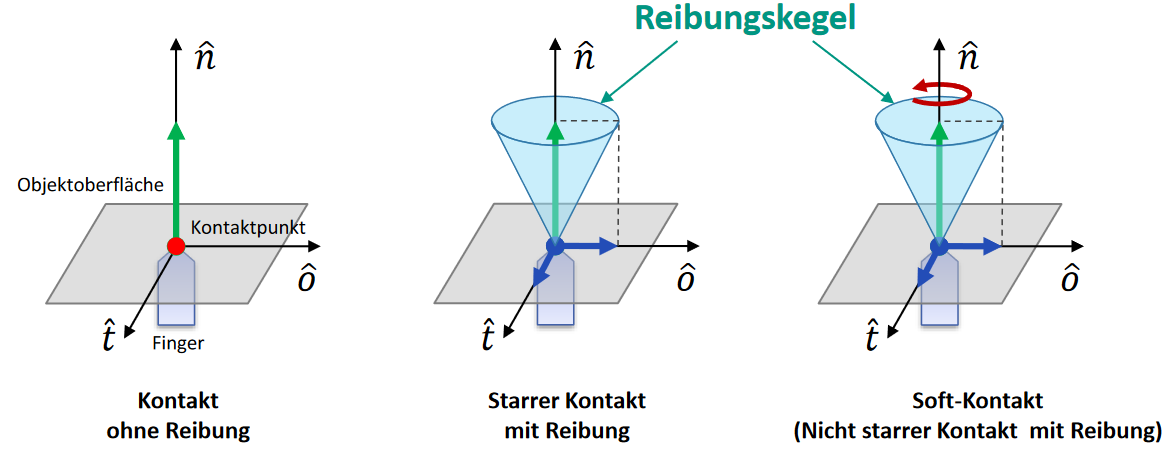
\includegraphics[width=0.7\textwidth]{images/kraftmodelle.png}
	\end{center}
	\item \textbf{Coulombsches Gesetz}: Beschreibt Verhältnis von tangentialer Kraft $f_t$ zu normaler Kraft $f_n$:
	$$f_t\leq\mu\cdot f_n$$
	mit \textbf{Reibungskoeffizient} $\mu>0$ abhängig vom Material
	\begin{center}
		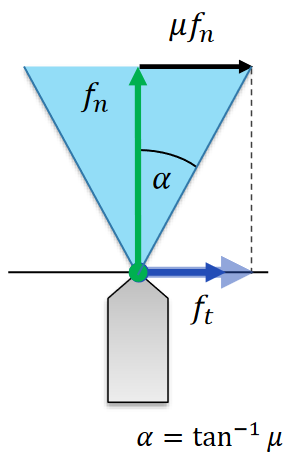
\includegraphics[width=0.15\textwidth]{images/coulomb.png}
	\end{center}
\end{itemize}
\bigskip
\textbf{Wrench}: Die in einem Kontaktpunkt $p$ wirkenden Kräfte $\mathbf{f}$ und Momente $\boldsymbol{\tau}$ können zu einem Wrench $\mathbf{w}$ zusammengefasst werden
\begin{itemize}
	\item Planarer Wrench (2D): $\mathbf{w}=\irow{f_x&f_y&\tau_z}^\top\in\R^3$
	\item Räumlicher Wrench (3D): $\mathbf{w}=\irow{f_x&f_y&f_z&\tau_x&\tau_y&\tau_z}^\top\in\R^6$
\end{itemize}
\bigskip
\textbf{Approximation des Reibungskegels}: Reibungskegel $WC\subseteq\R^6$ ist die \textbf{positive lineare Hülle} der $w_i$:
$$WC=\{\sum\limits_{i=1}^{n} k_iw_i\mid k_i\geq 0\}$$
\begin{center}
	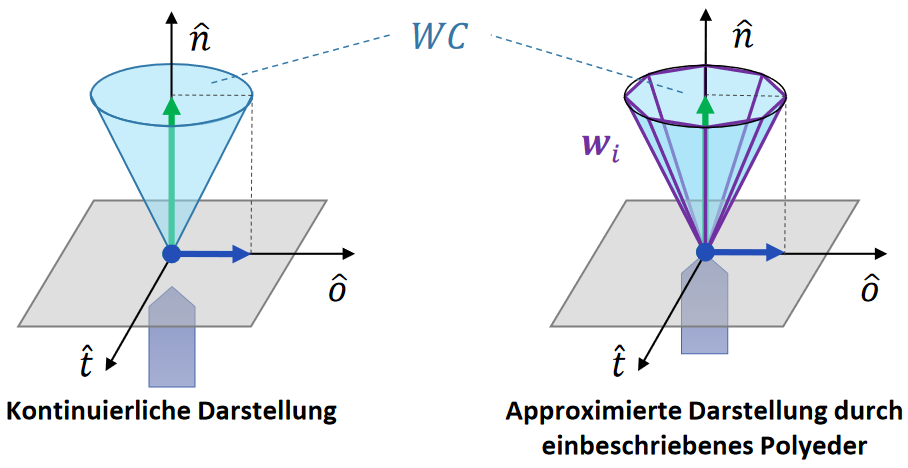
\includegraphics[width=0.7\textwidth]{images/polyeder.png}
\end{center}

\textbf{Stabilität eines Griffs}:
\begin{itemize}
	\item \textbf{Gleichgewichtsgriff}: Summe aller Kräfte und Momente, die auf das gegriffene Objekt wirken, ist 0: $\mathbf{w}_\text{ext}+\sum\limits_{i} \mathbf{w}_i=0$
	\item \textbf{Kraftgeschlossene Griffe}: 
	\begin{itemize}
		\item \textbf{Annahme}: Kontakte können beliebig große Kräfte ausüben
		\item \textbf{Frage}: Kann der Griff beliebigen externen Wrenches entgegenwirken? 
		\item Griff ist \textbf{kraftgeschlossen}, wenn $WC=\R^d$ gilt, wobei $WC$ die positive lineare Hülle der einzelnen Reibungskegel ist $\rightarrow$ Dann können Wrenches in alle Richtungen erzeugt werden
		\item \textbf{Beispiel}: \textit{8/39-40}
	\end{itemize}
	\item \textbf{Greifmatrix}: Seien $\mathbf{w}_1,\ldots,\mathbf{w}_m\in\R^6$ die Wrenches, die die Reibungskegel aller Kontakte aufspannen. Greifmatrix $G$ enthält die Wrenches aller Reibungskegel als Spalten:
	$$G=\left(
	\begin{matrix}
		 &  \\
		\mathbf{w}_1   & \cdots & \mathbf{w}_m  \\
		 & 
	\end{matrix}
	\right)\in\R^{6\times m}$$
	\begin{itemize}
		\item Griff ist \textbf{kraftgeschlossen}, wenn $G$ vollen Rang hat und es ein $\mathbf{k}=\irow{k_1 & \cdots & k_m}$ mit $k_j>0$ gibt, sodass $G\cdot\mathbf{k}=0$
	\end{itemize}
	\item \textbf{Formgeschlossene Griffe}: 
	\begin{itemize}
		\item \textbf{Frage}: Kann der Griff beliebigen externen Wrenches entgegenwirken, wenn keine Reibung existiert?
		\item Antwort wie bei kraftgeschlossenen Griffen, aber nur Berücksichtigung von Kräften entlang der Normalen
		\item \textbf{Beispiel}: \textit{8/44-45}
	\end{itemize}
	\item Um $\R^d$ positiv aufzuspannen, sind $d+1$ Vektoren nötig
	\item Formgeschlossene Griffe $\subseteq$ Kraftgeschlossene Griffe $\subseteq$ Gleichgewichtsgriffe
\end{itemize}
\bigskip
\textbf{Griffqualität}:
\begin{itemize}
	\item Beide Griffe sind kraftgeschlossen, aber sind beide auch gleich gut?
	\begin{center}
		\includegraphics[width=0.4\textwidth]{images/qualität.png}
	\end{center}
	\item \textbf{Grasp-Wrench-Space}: Seien $\mathbf{w}_1,\ldots,\mathbf{w}_m\in\R^6$ die Vektoren, die die Reibungskegel aller Kontakte approximieren. $GWS$ ist die konvexe Hülle der $\mathbf{w}_i$
	$$GWS=\{\sum\limits_{i=1}^{m}k_i\mathbf{w}_i\mid k_i\geq 0 \text{ und } \sum\limits_{i=1}^{m} k_i=1\}$$
	\begin{center}
		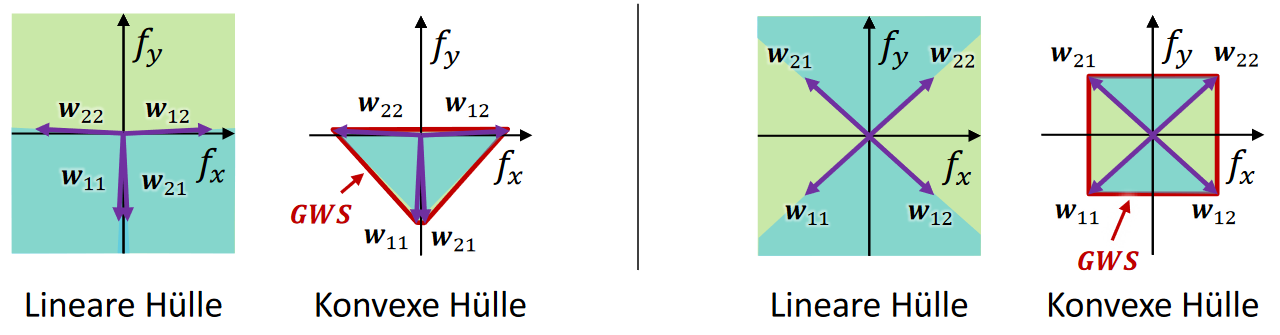
\includegraphics[width=0.7\textwidth]{images/gws.png}
	\end{center}
	\item \textbf{$\boldsymbol{\varepsilon}$-Metrik}: ist der Radius der größten Kugel um den Ursprung des $GWS$, die noch vollständig in $GWS$ enthalten ist
	\begin{center}
		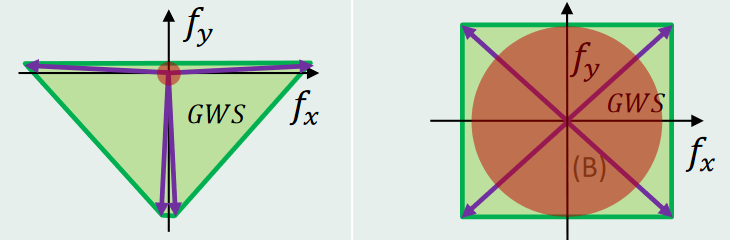
\includegraphics[width=0.4\textwidth]{images/epsilon.png}
	\end{center}
	$\rightarrow$ Griff B ist besser
\end{itemize}
\bigskip
\textbf{Klassifikation von Greifplanungssystemen}:
\begin{itemize}
	\item Typ des Greifers, Typ der Sensorik
	\item Typ der zugrunde liegenden Greifplanungsalgorithmen
	\item Typ der Geometrie des zu greifenden Objekte
\end{itemize}
\bigskip
\textbf{Objektklassen für das Greifen}:
\begin{itemize}
	\item \textbf{Bekannte Objekte}
	\item \textbf{Bekannte Objektklasse}: Konkrete Objektgeometrie ist nicht bekannt
	\item \textbf{Unbekannte Objekte}
\end{itemize}
\bigskip
\textbf{Definition eines Griffes}: Griff kann definiert werden durch
\begin{itemize}
	\item Griffmittelpunkt auf dem Objekt
	\item Annäherungsvektor beschreibt den Winkel mit dem sich die Hand dem Griffmittelpunkt nähert 
	\item Orientierung des Handgelenks
	\item Initiale Fingerkonfiguration
\end{itemize}
\bigskip
\textbf{Griffsynthese durch Vorwärtsplanung}:
\begin{itemize}
	\item Planung in Simulation
	\item Bestimmung von Anfahrtspunkt und Anfahrtsrichtung
	\item Hand nähert sich dem Objekt, bis ein Kontakt detektiert wird. Finger schließen sich um das Objekt, bis Kontakt hergestellt ist
	\item Evaluation der Kontakte zwischen Hand und Objekt
\end{itemize}
\bigskip
\textbf{Zufallsbasierte Vorwärts-Greifplanung}:
\begin{enumerate}
	\item Randomisierte Erzeugung von Griffhypothesen
	\item Kontaktermittlung
	\item Evaluation der Hypothesen
\end{enumerate}

Objekte werden durch einfache \textbf{Formprimitive} wie \textbf{Boxen} oder \textbf{Superquadriken} dargestellt. \textbf{Box-Dekomposition} führt zu einer besseren Approximation bei box-basierten Ansätzen.\\

\textbf{Griffplanung mit medialen Achsen}: \textit{8/97-128}
\pagebreak